\documentclass[a4paper, 12pt]{article}

\usepackage[T1]{fontenc}
\usepackage[utf8]{inputenc}
%\usepackage{lmodern}
%\usepackage{hyperref}
\usepackage{nohyperref} % This makes hyperref commands do nothing without errors
\usepackage{url}
\usepackage{graphicx}
\usepackage{seqsplit} 
\usepackage{varioref} % for vref
\usepackage{tabularx}
\usepackage{tabulary}
\usepackage{enumerate}
\usepackage[acronym]{glossaries}

\newacronym{nhs}{NHS}{National Health Service}
\newacronym{tds}{TDS}{Traffic Distribution Software}
\newacronym{candc}{C\&C}{Command-and-Control}

\makeglossaries

% Variables
\renewcommand{\title}{Ransomware: A systematic overview}
\renewcommand{\author}{Jan Schlenker}

\newcommand{\tabitem}{~~\llap{\textbullet}~~}

\setlength{\parindent}{0pt} % no indent after figure
\setlength{\skip\footins}{1cm} % indent before footnote

% ******************** BEGIN OF DOCUMENT ********************
\begin{document}

\begin{titlepage}

\newcommand{\HRule}{\rule{\linewidth}{0.5mm}} % Defines a new command for the horizontal lines, change thickness here

\center % Center everything on the page
 
%----------------------------------------------------------------------------------------
%	HEADING SECTIONS
%----------------------------------------------------------------------------------------

\textsc{\LARGE University of Innsbruck}\\[1.5cm] % Name of your university/college
\textsc{\Large Seminar Work}\\[0.5cm] % Major heading such as course name
\textsc{\large Master Seminar 2 (703606 SE/2)}\\[0.5cm] % Minor heading such as course title

%----------------------------------------------------------------------------------------
%	TITLE SECTION
%----------------------------------------------------------------------------------------

\HRule \\[0.4cm]
{ \huge \bfseries \title}\\[0.4cm] % Title of your document
\HRule \\[1.5cm]
 
%----------------------------------------------------------------------------------------
%	AUTHOR SECTION
%----------------------------------------------------------------------------------------

\begin{center}
\begin{tabular}{l l}
Author: & \author \\
Supervisor: & Christian Sillaber \& Clemens Sauerwein \\
Semester: & SS 2016/2017
\end{tabular}
\end{center}

% If you don't want a supervisor, uncomment the two lines below and remove the section above
%\Large \emph{Author:}\\
%John \textsc{Smith}\\[3cm] % Your name

%----------------------------------------------------------------------------------------
%	DATE SECTION
%----------------------------------------------------------------------------------------

%{\large \today}\\[3cm] % Date, change the \today to a set date if you want to be precise

%----------------------------------------------------------------------------------------
%	LOGO SECTION
%----------------------------------------------------------------------------------------

%\includegraphics{Logo}\\[1cm] % Include a department/university logo - this will require the graphicx package
 
%----------------------------------------------------------------------------------------

\vfill % Fill the rest of the page with whitespace

\end{titlepage}

%\include{01_abstract}

\tableofcontents
\newpage

\printglossary[title=List of Acronyms, type=\acronymtype]
\listoffigures
\listoftables

\section{Introduction}

Ransomware is one of the biggest cybercrime threats of our days, both for organizations and individuals. This was again demonstrated by the recent global attack of the WannaCry trojan \cite{Symantec2017} shown in figure \ref{fig:wanna_cry}, where more than 230000 computers in 150 different countries got infected. The attack also showed that there is often still no other way for infected victims than paying the ransom, if they want to get their data back and have no sufficient Backups. Precautions like regular security updates can help to avoid the damage, but there is no waterproof solution and people working with crucial data need to be educated about the topic. Among others, the \gls{nhs} faced huge troubles through WannaCry \cite{Martin2017}, which exemplifies that wallets can be affected by ransomware as well as health conditions.

\begin{figure}[htbp]
  \begin{center}
    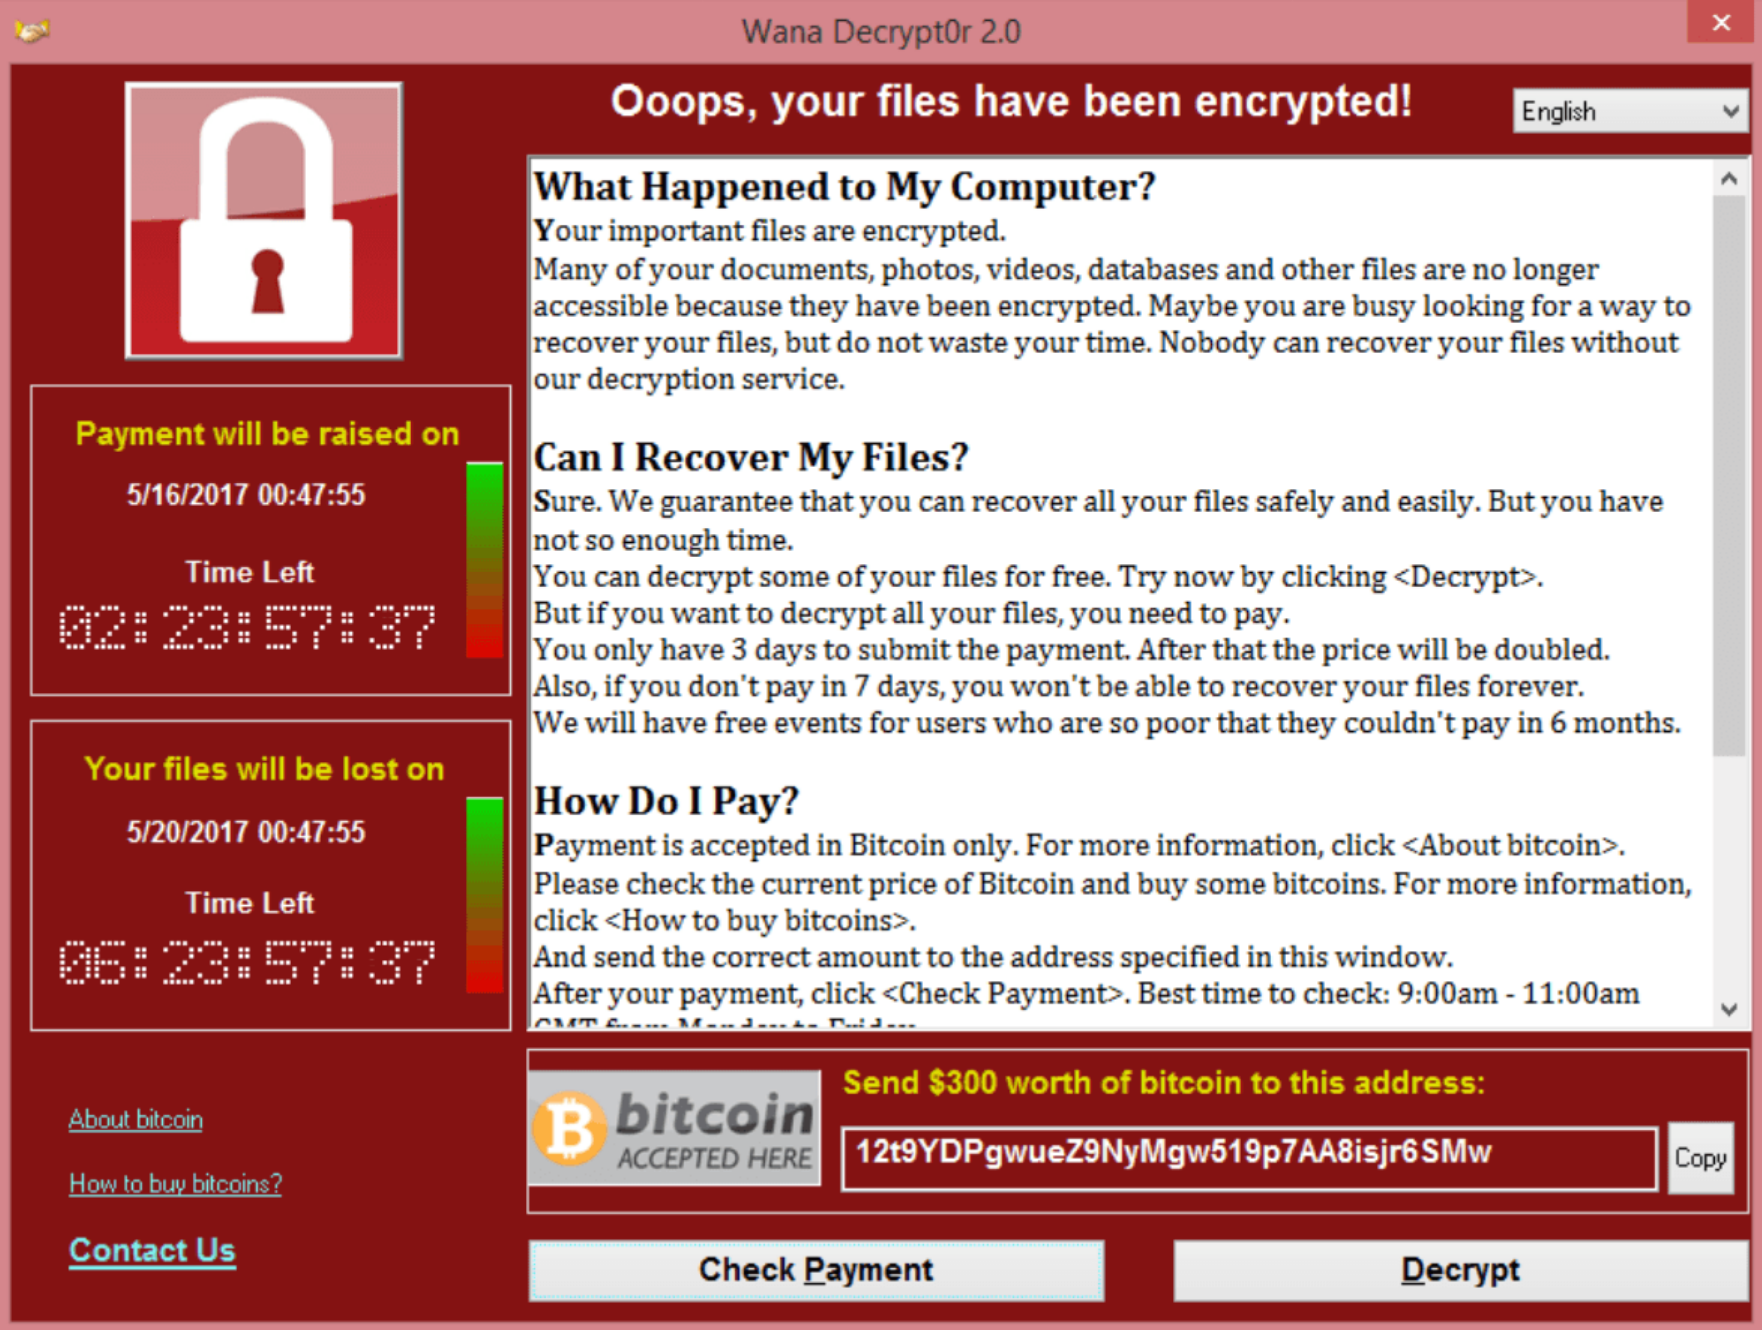
\includegraphics[width=0.8\textwidth]{images/wanna_cry.png}
    \caption{WannaCry Ransomware}
    \label{fig:wanna_cry}
  \end{center}
\end{figure}

This seminar work focuses on giving an overview of ransomware.
%TODO

\section{What is Ransomware?}

Ransomware in general is a malicious software, that denies access to the files of the victim or/and threatens to publish them. Most of the time it is distinguished by researchers into 2 major types:

\begin{description}
\item[File lockers:] The most common ransomware type, also known as ``crypto trojan'' or ``crypto ransomware''. Here the files of the victim are usually encrypted and the attacker demands the ransom for the decryption. Some variants do not encrypt the files but deny the access to the files in some other way, for example by putting them into a password protected archive \cite{Symantec2017a}.
  
\item[Screen lockers:] Here the victims access to its system is denied, mostly by changing the password or the pin. In this case the attacker demands the ransom for the new authentication code.
\end{description}

Pure screen lockers are not as dangerous as file lockers, because the (personal) files of the victim are not touched and can be recovered by accessing the harddrive from another system. However, file and screen lockers can be combined, which would prevent this recovering technique.\\
\\
Some sources name ``Leakware'' also known as ``Doxware'' as a third ransomware type \cite{Upadhaya2017}, where the attacker demands the ransom for not publishing the data of the victim. Companies can be targets, which do not want to share crucial data with their competitors, but also individuals, which for example have intimate photos on their device. Likewise this type can be combined with screen and file lockers.\\
\\
In contrast to other malware, ransomware reveals itself to the victim at some point (e.g. when the files are encrypted). Traditional malware rather aims to achieve stealth for collecting banking credentials or keystrokes without raising suspicion \cite{Kirda2017}. Ransomware on the other hand wants to get the attention of the victim to demand the ransom.


\bibliographystyle{unsrt}
\bibliography{bibliography}

\section*{Declaration of Authorship}

\noindent I, \emph{\author}, declare that this seminar work titled \emph{\title} and the work presented in it are my own. I confirm that:

\begin{itemize} 
\item Where I have consulted the published work of others, this is always clearly attributed.
\item Where I have quoted from the work of others, the source is always given. With the exception of such quotations, this seminar paper is entirely my own work.
\item I have acknowledged all main sources of help.
\end{itemize}
 
\noindent Signed:\\
\rule[0.5em]{25em}{0.5pt} % This prints a line for the signature
 
\noindent Date:\\
\rule[0.5em]{25em}{0.5pt} % This prints a line to write the date


\end{document}
% ******************** END OF DOCUMENT ********************
